\newpage
\chapter{METODE PENELITIAN} \label{Bab III}

\section{Alur Penelitian} \label{III.Alur}
% Pada penelitian ini, alur dirancang untuk memastikan setiap tahapan pemrosesan dilakukan secara sistematis dan efisien. Alur penelitian ini mencerminkan langkah-langkah utama yang dilakukan pada penelitian ini, dapat dilihat pada Gambar \ref{fig:3.alur}. \par
Penelitian ini dilakukan dengan pendekatan kuantitatif eksperimental yang berfokus pada penerapan metode deep learning, khususnya arsitektur Text CNN, untuk klasifikasi sentimen komentar cyberbullying. Secara umum, alur penelitian ini terdiri dari beberapa tahapan utama, yaitu: \par

\begin{figure}[H] % Kalau menggunakan H, posisi gambar akan tepat dibawah teks
    \centering
    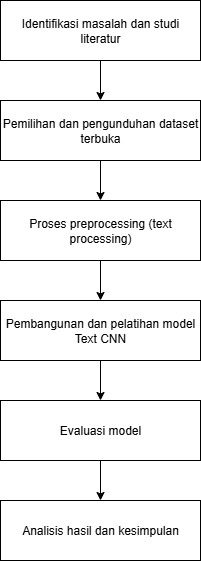
\includegraphics[width=0.3\textwidth]{figure/sistematika-penelitian.jpg}
    \caption{Alur Penelitian}
    \label{fig:3.alur}
\end{figure}

\section{Penjabaran Langkah Penelitian} \label{III.Jabar Alur}
Untuk memperjelas setiap langkah-langkah yang telah didefinisikan pada Gambar \ref{fig:3.alur}, berikut ini akan dijelaskan secara rinci tahapan-tahapan yang dilakukan dalam penelitian ini.

\subsection{Identifikasi Masalah} \label{III.Identifikasi_masalah}
% \lipsum[1] % Menampilkan paragraf 1 sampai 2 dari lorem ipsum


\section{Alat dan Bahan Tugas Akhir} \label{III.Alat dan Bahan}
Dalam menjalani penelitian, beberapa alat dan bahan digunakan untuk memastikan penelitian berjalan dengan baik.\par

\subsection{Alat} \label{III.Alat}
Dalam menganalisis sentimen komentar cyberbullying pada TikTok menggunakan arsitektur Text CNN, berikut adalah alat-alat yang digunakan: \par

\subsubsection{Perangkat Lunak}
\begin{enumerate}[noitemsep]
    \item \textit{Visual Studio Code} sebagai \textit{text editor}.
    \item Torch versi 2.3.1
    \item transformers versi 4.51.2
    \item NumPy versi 1.26.2
    \item Pandas versi 2.2.3
    \item Scikit-learn versi 1.7.0
    \item Matplotlib versi 3.9.0
    \item Wandb versi 0.19.11
    \item Tqdm versi 4.66.5
    \item Muon-optimizer versi 0.1.0
\end{enumerate}

\subsubsection{Perangkat Keras}
\begin{itemize}[noitemsep]
	\item Asus Vivobook 14x m1403qa
    \item Processor AMD Ryzen 5 5600H with Radeon Graphics    
    \item RAM 24 GB
    \item AMD Radeon (TM) Graphics
    \item Sistem operasi Windows 11 Home 64-bit
\end{itemize}

\subsection{Bahan} \label{III.Bahan}
Dataset yang digunakan pada penelitian ini merupakan dataset komentar TikTok yang diperoleh dari repositori GitHub penelitian Prameswari et al \cite{10468424}. Dataset ini berisi komentar-komentar TikTok yang telah dilabeli dengan kategori sentimen positif dan negatif. Dataset ini berisi 1.508 data komentar TikTok yang telah dilabeli. Dataset ini digunakan untuk melatih dan menguji model Text CNN dalam mengklasifikasikan sentimen komentar TikTok yang mengandung unsur cyberbullying.

\section{Ilustrasi Perhitungan Metode} \label{III.Ilustrasi}
Metode yang digunakan dalam penelitian ini adalah Text CNN (Text Convolutional Neural Network), yaitu arsitektur CNN yang diadaptasi untuk klasifikasi teks. Berikut tahapan dan ilustrasi metode: \par

\subsection{Embedding Layer}
Komentar yang telah diproses diubah menjadi vektor representasi kata (menggunakan Word2Vec, GloVe, atau embedding trainable). \par
Misal: \texttt{"kamu jelek"} → \texttt{[[0.2, -0.4], [0.5, 0.7]]}

\subsection{Convolutional Layer}
Filter konvolusi diterapkan untuk mengekstrak pola n-gram.
Misal filter size: 2, 3, 4.

\subsection{ReLU Activation Function}
Fungsi aktivasi ReLU digunakan untuk menambah non-linearitas.

\subsection{Max Pooling}
Memilih nilai fitur tertinggi dari hasil konvolusi untuk mempertahankan fitur paling signifikan.

\subsection{Fully Connected Layer}
Output pooling digabung dan diteruskan ke dense layer.

\subsection{Output Layer}
Fungsi aktivasi softmax digunakan untuk mengklasifikasikan komentar ke dalam salah satu kelas: positif, netral, atau negatif.

% Dalam penelitian ini, hasil perhitungan dari program akan melalui serangkaian pengujian untuk mengevaluasi tingkat keakuratan model yang digunakan. Data dummy tersebut dapat dilihat pada Tabel \ref{table:3.dummy}. \par
% \begin{longtable}{|c|c|c|c|c|c|c|c|c|}
% 	\caption{Data \textit{dummy} Pengujian}
% 	\label{table:3.dummy}\\
% 	\hline
% 	\multirow{2}{*}{\textbf{Subjek}} & \multicolumn{7}{|c|}{\textbf{Hasil Prediksi (BPM)}} & \multirow{2}{*}{\textbf{GT}} \\ \cline{2-8}
%     & \textbf{F} & \textbf{NA} & \textbf{NO} & \textbf{RC} & \textbf{LC} & \textbf{M} & \textbf{C} & \\ 
%         \hline
% 	   \endfirsthead
%        \hline
%        \multirow{2}{*}{\textbf{Subjek}} & \multicolumn{7}{|c|}{\textbf{Hasil Prediksi (BPM)}} & \multirow{2}{*}{\textbf{GT}} \\ \cline{2-8}
%     & \textbf{F} & \textbf{NA} & \textbf{NO} & \textbf{RC} & \textbf{LC} & \textbf{M} & \textbf{C} & \\ 
%     \hline
% 	\endhead
% 	\hline
% 	\endfoot
% 	\hline
% 	\endlastfoot
% 	1 & 68 & 69 & 68 & 70 & 68 & 71 & 69 & 68 \\ 
% 	\hline
% 	2 & 69 & 69 & 68 & 70 & 68 & 71 & 69 & 69 \\
% 	\hline
% 	3 & 70 & 70 & 69 & 71 & 68 & 73 & 69 & 70\\
% 	\hline
% 	4 & 71 & 70 & 70 & 72 & 69 & 73 & 70 & 71 \\
% 	\hline
% 	5 & 72 & 72 & 70 & 72 & 70 & 74 & 70 & 72 \\
% 	\hline
%         6 & 73 & 72 & 71 & 74 & 71 & 76 & 71 & 73 \\ 
% 	\hline
% 	7 & 74 & 73 & 72 & 74 & 72 & 77 & 71 & 74 \\
% 	\hline
% 	8 & 75 & 74 & 72 & 74 & 73 & 77 & 73 & 75\\
% 	\hline
% 	9 & 76 & 75 & 73 & 75 & 74 & 78 & 75 & 76 \\
% 	\hline
% 	10 & 77 & 76 & 74 & 78 & 75 & 78 & 76 & 77
% \end{longtable}